\documentclass[]{report}
\usepackage{helvet}
\usepackage{graphicx,wrapfig,lipsum}
\usepackage[export]{adjustbox}
\usepackage{fullpage}
\usepackage{sectsty}
\setcounter{secnumdepth}{3}
\chapterfont{C}  % sets colour of chapters
\sectionfont{\color[HTML]{575775}}  % sets colour of sections
\subsectionfont{\color[HTML]{474785}} 
\subsubsectionfont{\color[HTML]{52527a}} 
\renewcommand{\familydefault}{\sfdefault}
\renewcommand{\baselinestretch}{2.0}
\setlength\parindent{24pt}
\usepackage[table,xcdraw]{xcolor}
\usepackage{indentfirst}
\usepackage{float}
\usepackage{titlesec}
\usepackage{booktabs}
\usepackage{caption}
\captionsetup{labelfont={color=gray},font={color=gray}}
\titleformat{\chapter}[hang] 
{\normalfont\huge\bfseries\centering\color[HTML]{42428a}}{\chaptertitlename\ \thechapter:}{1em}{} 
%\usepackage[backend=bibtex,style=authoryear,bibstyle=authoryear,sorting=nyt,firstinits=true]{bibla%tex}
% Title Page

%\addbibresource{sample.bib} 
\title{3D Motor Expolorer}
\author{Firas \& Slim}


\begin{document}
\maketitle
\tableofcontents
\listoffigures
\listoftables

\newpage
\chapter{Presentation}
\section{Introduction}
 The following work is part of our graduation project for the applied bachelor
	degree in Information System Development at XTech . This internship tasked us
	with the realization of a web VR application named : Motor Explorer .
	This Chapter will contain the hosting company introduction followed by
	primary studies we ran before getting to work on the project , leading into
	detailed explanation of our solution and eventually we will talk about the
	methodology used to realize this project .

\section{Hosting organization Presentation}
\begin{figure}[H]
	\begin{center}
	
\includegraphics[scale=0.5]{XTECHLogo.png}
	\caption{XTECH Logo}
	\end{center}
\end{figure} \par



xTECH is an is an up-and-coming tech company based between Berlin and Tunis, developing web applications and cloud solutions. They help connect talented developers with innovative clients in order to create high quality solutions.\par


\section{Preliminary studies}
In this section we will discuss the origins of webVR and the pros and cons
about webVR in general.
\subsection{WEB VR}
\subsubsection{Definition and history }
WebVR was an experimental JavaScript API that allowed web applications to
	interact with VR devices like the “HTC Vive” , “Ouclus rift” , “Google
	cardboard” and such . It was first conceived in early spring 2014 by “Vladimir
	Vukićević” from “Mozilla” and on March 2016 “Google Chrome” and the
	2
	“Mozilla VR” team announced the version 1.0 which by April 2017 was
	upgraded to version 1.1 and by than companies like Microsoft joined in on the
	project and are actively collaborating on the 2.0 version \cite{lambo}

\subsubsection{Goals}

The API was designed with these goals in mind:
\begin{itemize}
	
		\item It works with all OS and devices
		\item webVR development is cheaper
		than native app for a single device
		\item A webVR App can be easily
		integrated into companies
		\item Can be used without installation
		\item WebVR Apps are updated instantly
		and no need to go though approval
		process
\end{itemize}
\subsubsection{Pros and cons}
\begin{table}[H]
	
 \begin{tabular}{|c| c|}
 	
	\hline
	\rowcolor[HTML]{6600ff}  \color{white}Pros & \color{white}Cons\\\hline
	\parbox{.45\textwidth}{\begin{itemize}
			\item It works with all OS and devices
			\item webVR development is cheaper
			than native app for a single device
			\item A webVR App can be easily
			integrated into companies
			\item Can be used without installation
			\item WebVR Apps are updated instantly
			and no need to go though approval
			process
	\end{itemize}} & \parbox{.45\textwidth}{\begin{itemize}
			\item Does not allow intense or
			complex 3D rendering
			\item It is difficult to navigate the app
			without the use of provided VR
			controllers
			\item Currently , webVR apps are still
			not as popular as native VR apps
			\item Requires more technical skills
			(Javascript in particular) experience
			than regular native VR apps
	\end{itemize}}\\\bottomrule
\end{tabular}
\caption[Pros and Cons of webVR]{Pros and Cons of webVR}
\end{table}
\subsubsection{Conclusion}
The trend is currently noticeably towards the WebVR app when it comes to
developing enterprise VR apps. This development is correct in that it puts more
emphasis on the price / performance ratio and less on the graphics quality.
3
WebVR apps are easy to integrate into existing IT structures and reduce manual
adjustment work for new end devices.

\section{Project goals}
The project’s goal is to help design a virtual reality environment which a
student or a worker can interact with on a physical level and understand the
mechanics behind the work they are tasked to do, it is meant to enhance the
level of understanding by providing a close to reality experience .

\section{Proposed solution}
Instead of using written documentation or 2D platforms, the user will have an
actual interface in which he can interact with and get a better understanding and
feeling to the experiment he is conducting and enhance the learning capacities
of students and give workers a better environment to work in
Therefor we will create a 3D simulator with sounds and visual 3D objects that
will keep the user entertained during his immersive experience while
conducting the task needed to be done and such solution will contain :
\begin{itemize}
	\item Development of a 3D environment
	\item Development of 3D motors
	\item Development of a 3D Dynamometer
	\item Development of a interactive Control-Pannel
	\item Development of real-life 3D animations
\end{itemize}

\section{Related Works}
\subsection{Motor explorer (original application)}
Motor explorer is the original application from which we have chosen to
migrate from a 2D platform to a 3D efficient platform for multiple reasons in
4
which we will mention below the different aspects from migrating from a
simple web solution to a complicated web VR environment in which the user
will have a more understanding of the purpose of the application.
Motor explorer is used to measure torque in a simulated experience the 2D
interface doesn’t offer much details toward this suggested test and this
application is used for only educational purposes as there would be no
professional aspect of the application .

\begin{figure}[H]
	\begin{center}
		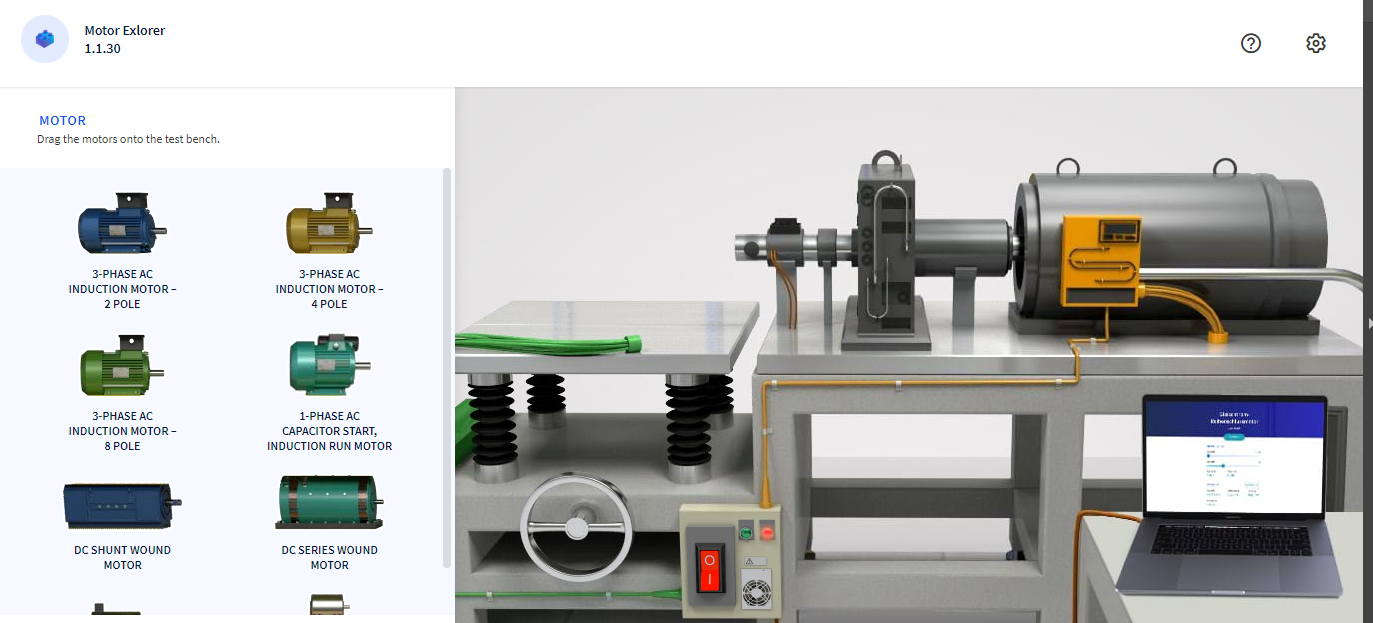
\includegraphics[scale=0.5, frame]{2dMotorExplorer.png}
	\end{center}
	\caption{2D Motor Explorer}
\end{figure}
As you see from the previous screenshot it’s the simple interface of the motor
explorer original application

\begin{table}[H]

	\begin{center}
	\begin{tabular}{|l|l|}
		\hline
		\rowcolor[HTML]{6600ff}
		\multicolumn{1}{|c|}{\color{white}Motor explorer 2D}                                     & \multicolumn{1}{c|}{\color{white}Motor Explorer web VR}                                                                          \\ \hline
		{\color[HTML]{009901} Simple 2D interface}                                  & {\color[HTML]{FE0000} 3D detailed interface}                                                                        \\ \hline
		{\color[HTML]{009901} Only drag-drop interactions}                          & {\color[HTML]{FE0000} \begin{tabular}[c]{@{}l@{}}User can interact in anyway with the\\ interface\end{tabular}}     \\ \hline
		{\color[HTML]{009901} No real-life experience can be felt during the tests} & {\color[HTML]{FE0000} \begin{tabular}[c]{@{}l@{}}Tests are conducted in a real-life like\\ experience\end{tabular}} \\ \hline
		{\color[HTML]{009901} Only for educational purposes}                        & {\color[HTML]{FE0000} Can also be applied in professional use}                                                      \\ \hline
	\end{tabular}
	\caption[Comparison between the 2d app and the 3d app]{Comparison between the 2d app and the 3d app}
\end{center}

\end{table}

\subsection{ESTPE VR}
ESTPE VR is designed for universities, training centers and organizations
providing professional development for the personnel at electric high-voltage
substations.
The main goal of this work is to improve the quality of training in electrical
engineering via implementation into the educational process a Virtual Reality
simulator developed specifically for the power industry of which we mention

\begin{itemize}
	\item Transformer Oil Sampling In Virtual Reality
\end{itemize}
The participants are able to perform field-job and familiarize themselves
with a transformer oil sampling procedure.
\begin{figure}[H]
	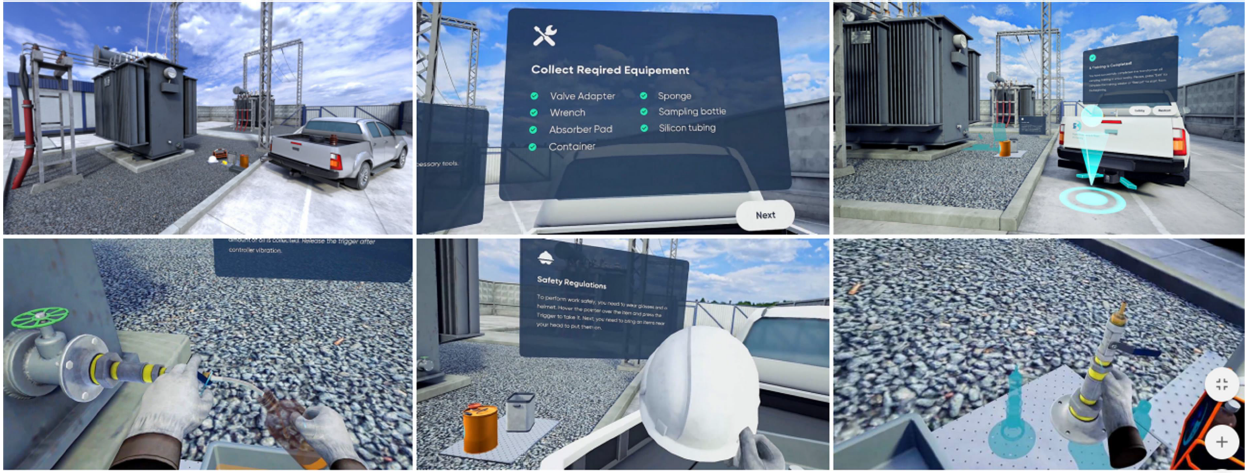
\includegraphics[scale=0.5]{ESTPEVR.png}
	\caption{Transformer Oil Sampling UI}
\end{figure}
\begin{itemize}
	\item Occupational Safety And Health Training for Electricians
\end{itemize}
This training is dedicated to maintaining safety at the workplace.
\begin{figure}[h]
	\begin{center} 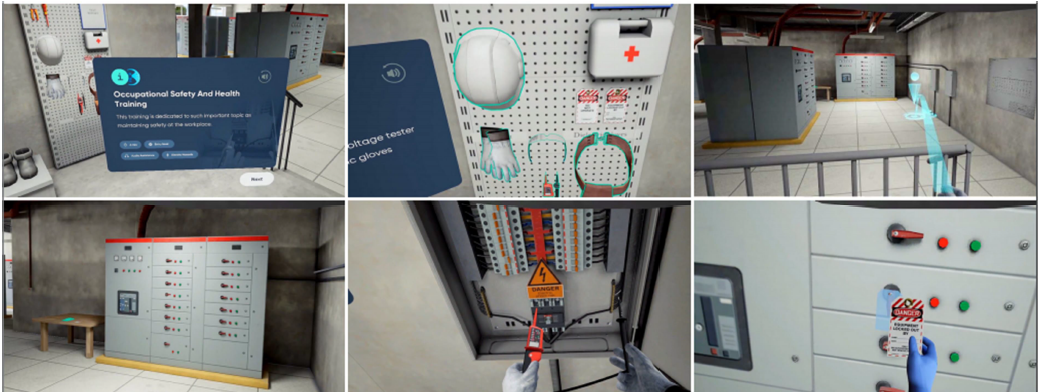
\includegraphics[scale=0.6]{ESTPEVR1.png}
	\caption{Occupational Safety And Health Training for Electricians UI}
	\end{center}
\end{figure}


{\Large{\color[HTML]{00D2CB} Comparison between  apps}}
\begin{table}[H]

	\begin{center}
	\begin{tabular}{|c|c|c|}
		\hline
		\rowcolor[HTML]{6600ff}
		{\color[HTML]{ffffff} }                   & {\color[HTML]{ffffff} ESTPE-VR}                     & {\color[HTML]{ffffff} Motor Explorer}              \\ \hline
		{\cellcolor[HTML]{6600ff}\color[HTML]{ffffff} Implements VR}      & {\color[HTML]{009901} YES}                          & {\color[HTML]{009901} YES}                         \\ \hline
		{\cellcolor[HTML]{6600ff}\color[HTML]{ffffff} Difficulty}         & {\color[HTML]{FE0000} Hard to use}                  & {\color[HTML]{009901} Easy to navigate}            \\ \hline
		{\cellcolor[HTML]{6600ff}\color[HTML]{ffffff} Required equipment} & {\color[HTML]{FE0000} Requires multiple VR gadgets} & {\color[HTML]{009901} Can be used without Headset} \\ \hline
		{\cellcolor[HTML]{6600ff}\color[HTML]{ffffff} Control system}     & {\color[HTML]{FE0000} Very hard to manipulate}      & {\color[HTML]{009901} Easy to navigate}            \\ \hline
		{\cellcolor[HTML]{6600ff}\color[HTML]{ffffff} Targeted audience}  & {\color[HTML]{FE0000} Only workers}                 & {\color[HTML]{009901} Both Students and workers}   \\ \hline
	\end{tabular}
\end{center}
	\caption[Comparison between our app and an existing app]{Comparison Comparison between our app and an existing app}
\end{table}

\section{Development Method}
The process of organizing a project and managing to deliver it in the right time
is a stressful and hard to manage process, you could encounter technical
problems that needs solving or conflict in the team responsible for the
development of the project. \\
Problems like these can be solved by using the agile methodology which we
will apply during the work on this project .

\subsection{Agile approach}

Agile consists of breaking the project into several stages which makes the
technical work more efficient and less sophisticated it also it involves the client
or in this case Product Owner with certain reviews at the end of each stage in a
way if a change is to bed made or an update is required it no longer requires to
start from scratch but to work on the stage in which the problem has been
encountered.

\subsection{Scrum Methodology}
The Scrum Methodology is the most common agile approach in which it
involves around three roles :
\begin{itemize}
	\item \large{\emph{The product owner}}
\end{itemize}
The Product owner is responsible behind organizing the requirements that the
project must meet, he also decides which functionalities get to be prioritized
during each stage of the development.

\begin{itemize}
	\item \large{\emph{The Team}}
\end{itemize}

The team is basically the members responsible of turning the project from idea
to an actual functioning product; they must respect the product backlog which is
set by the product owner. The team’s size must be as small as possible to avoid
conflicts and contradictory work ideas due to the different roles.

\begin{itemize}
	\item \large{\emph{The Scrum Master}}
\end{itemize}

The Scrum Master is basically the SCRUM itself, he must master it in all
different aspects and in a proper way. He ensures that the team is implementing
SCRUM in its proper ways in final words his job consists of organizing the
perfect flow between the team, their tasks, and the project manager.\\ \\
\textbf{Sprint:} The following is a diagram that will help understand that each Stage we
refer to as “Sprint”, throughout the workflow each sprint has its own updated
backlog, review and goal.

\begin{figure}[H]
	\begin{center}
	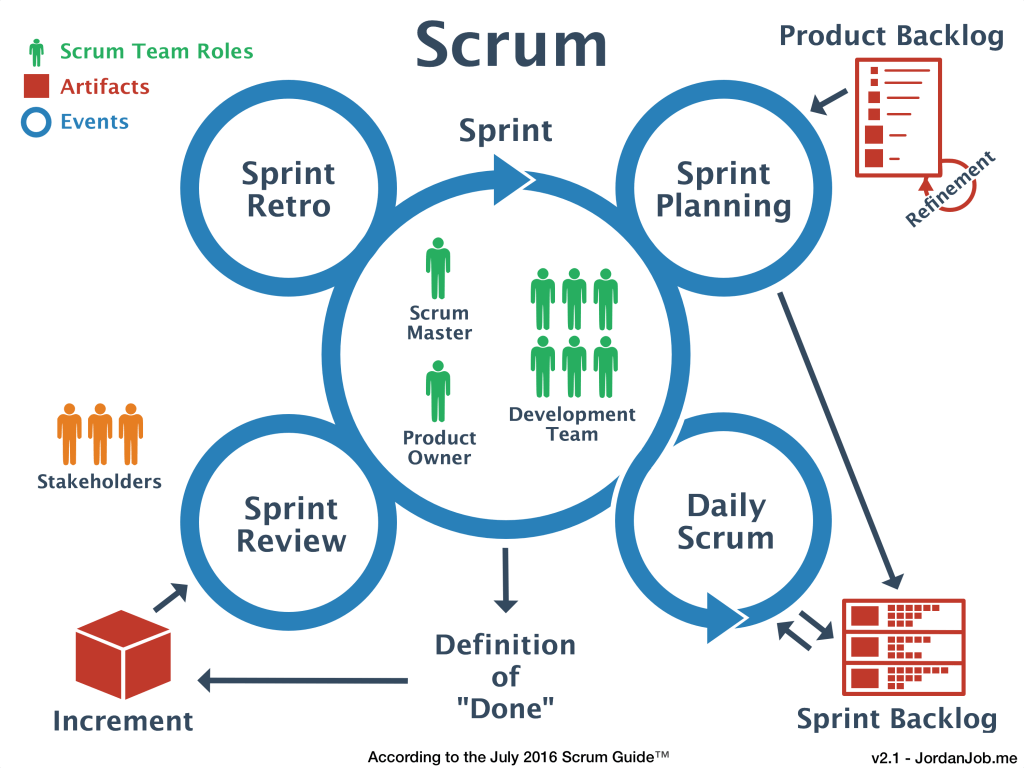
\includegraphics[width=150mm, frame]{scrum.png}
	\caption{Scrum explanation}
\end{center}
\end{figure}


To summarize, SCRUM’s bread and butter is composed of four keywords:
\begin{itemize}
	\item Sprint Planning:
\end{itemize}

Setting the different goals that the team believes is able to achieve during the set
period of a sprint.

\begin{itemize}
	\item Daily SCRUM
\end{itemize}

The daily SCRUM is a basically a small quick meeting which contains three
parts which are what was achieved the previous day, goals set for the current
day and discuss work blockers which are preventing certain progress.

\begin{itemize}
	\item Sprint Review
\end{itemize}

The sprint review is conducted at the end of each sprint, in which the they
approve certain completion of set tasks by consulting the backlog and also
provide a small demonstration of each completed task.

\begin{itemize}
	\item Sprint Review
\end{itemize}

The sprint retrospective is a meeting which the SCRUM team conducts to
discuss certain changes that emerge during the work; it also helps improving the
product itself and discusses certain updates to be made.

\section{Conclusion}
This chapter contained information about the hosting company XTECH. It also
provided a general definition of the project by discussing the main goal of the
proposed solution, ending it by choosing the development methodology to
follow throughout the realization of such project. In the next chapter we will
provide our analysis conducted prior to the development.






\chapter{Requirement analysis and specification}
\section{Introduction}
In this chapter we will discuss some of the analysis conducted
to deduce the requirements and specification conerning the
following project. We will lead by giving a brief definition to
our SCRUM roles and actors, and then we will follow by
requirements identification into product backlog and we will
close by showing the sprint planning and some general
modelisation .
\section{SCRUM Roles}
The scrum team is made of a product owner , the development
team and a scrum master. You will notice in our case that both
the scrum master and product owner roles are occupied by the
same person
\begin{itemize}
	\item Product owner / Scrum Master: Mr. Zied ben haj salah .
	He is responsible for making a decent presentation about
	the product characteristics and functionalities he also is
	responsible for the approval of the product development.
	His tasks as a SCRUM master are basically a supervision
	of the work progress, managing the team activities and
	organizing the meetings.
	\item The TEAM: Slim Bardaoui and Firas Bouadila they are
	in charge of delivering each sprint and the technical work
	as in the development.
\end{itemize}

\begin{table}[H]
	\begin{center}
	\begin{tabular}{cc}
		\hline
		
		\multicolumn{1}{|c|}{\cellcolor[HTML]{5900b3}\color[HTML]{f0e6ff}\textbf{Role}} & \multicolumn{1}{c|}{\cellcolor[HTML]{5900b3}\color[HTML]{f0e6ff}\textbf{Description}}           \\ \hline
		\multicolumn{1}{|c|}{Product Owner} & \multicolumn{1}{c|}{Zied bel haj salah}             \\ \hline
		\multicolumn{1}{|c|}{Scrum Master}  & \multicolumn{1}{c|}{Zied bel haj salah}             \\ \hline
		\multicolumn{1}{|c|}{Team}          & \multicolumn{1}{c|}{Firas bouadila , Slim Bardaoui} \\ \hline \multicolumn{1}{l}{}                               
	\end{tabular}
\end{center}
\caption[Scrum team]{Scrum team}
\end{table}

\section{Actors identification}
In general cases an actor is the targeted individual or
system to make use of the application or the solution
services. It conducts the general operations on the
application and in our case the actor would be:


\begin{table}[H]
	\begin{center}
		\begin{tabular}{|  p{5cm}  |  p{7cm} | }
			\toprule
			\raisebox{-\totalheight}{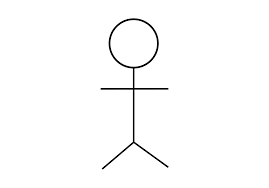
\includegraphics[width=0.3\textwidth, height=60mm]{User.png}}
			\centering User
			& Since our proposed solution
			doesn’t require any
			complicated interaction we
			will only have a single user
			who will make use of the
			immersive experience in the
			VR environment his tasks
			are :
			\begin{itemize}
				\item Pick the required motor
				\item Initiate the test
				\item Set the correct values
				needed 
				\item Take notes of the
				obtained results
			\end{itemize}
			\\ \bottomrule
		\end{tabular}
	\end{center}
\caption[Actors identification]{Actors identification}
\end{table}

\section{Requirements Identification}
In this section we will take a look at how we can transform
the basic goals of the project into a set of functions which
can be developed.
After having identified the main actor behind our
application, we will talk about functional and non-
Role Description
Product Owner Zied bel haj salah
Scrum Master Zied bel haj salah
Team Firas bouadila , Slim
Bardaoui
functional requirements followed by a use case diagram
explaining the global actions of our product.

\subsection{Functional Requirements}
\begin{itemize}
	\item Must provide accurate calculations
	\item Enable user to have detailed information about each
	motor
	\item Must provide a guided interface
\end{itemize}

\subsection{Non functional requirements}
\begin{itemize}
	\item The interface should be user friendly
	\item The graphics must be smooth
	\item Provide animations
	\item Provide inetractive noises
\end{itemize}
\section{Product backlog}

\begin{table}[H]
	\renewcommand{\arraystretch}{4} % this reduces the vertical spacing between rows
	\linespread{0.45}\selectfont\centering
	\begin{center}
	\begin{tabular}{ccc}
		\hline
		\rowcolor[HTML]{6600ff}
		\multicolumn{1}{|c|}{\color{white}\textbf{User story}}                                                                                                             & \multicolumn{1}{c|}{\color{white}\textbf{Priority}} & \multicolumn{1}{c|}{{\color{white}\textbf {Estimation(days)}}} \\ \hline
		\multicolumn{1}{|c|}{I as a user would like to see a control panel}                                                                                   & \multicolumn{1}{c|}{1}                 & \multicolumn{1}{c|}{1}                \\ \hline
		\multicolumn{1}{|c|}{I as a user would like to set the load}                                                                                          & \multicolumn{1}{c|}{2}                 & \multicolumn{1}{c|}{3}                \\ \hline
		\multicolumn{1}{|c|}{I as a user would like to set the speed}                                                                                         & \multicolumn{1}{c|}{3}                 & \multicolumn{1}{c|}{3}                \\ \hline
		\multicolumn{1}{|c|}{I as a user would like to set the voltage}                                                                                       & \multicolumn{1}{c|}{4}                 & \multicolumn{1}{c|}{3}                \\ \hline
		\multicolumn{1}{|c|}{I as a user would like to turn the test on and off}                                                                              & \multicolumn{1}{c|}{5}                 & \multicolumn{1}{c|}{2}                \\ \hline
		\multicolumn{1}{|c|}{I as a user would like to have a results menu}                                                                                   & \multicolumn{1}{c|}{6}                 & \multicolumn{1}{c|}{2}                \\ \hline
		\multicolumn{1}{|c|}{I as a user would like to have a motor menu}                                                                                     & \multicolumn{1}{c|}{7}                 & \multicolumn{1}{c|}{2}                \\ \hline
		\multicolumn{1}{|c|}{I as a user would like to see a dynamometer}                                                                                     & \multicolumn{1}{c|}{8}                 & \multicolumn{1}{c|}{2}                \\ \hline
		\multicolumn{1}{|c|}{I as a user would like to see a work-bench}                                                                                      & \multicolumn{1}{c|}{9}                 & \multicolumn{1}{c|}{2}                \\ \hline
		\multicolumn{1}{|c|}{I as a user would like to interact with the work-bench}                                                                          & \multicolumn{1}{c|}{10}                & \multicolumn{1}{c|}{8}                \\ \hline
		\multicolumn{1}{|c|}{\begin{tabular}[c]{@{}c@{}}I as a user would like to see the motors running\end{tabular}}                                      & \multicolumn{1}{c|}{11}                & \multicolumn{1}{c|}{2}                \\ \hline
		\multicolumn{1}{|c|}{\begin{tabular}[c]{@{}c@{}}I as a user would like to hear sounds indicating motor status\end{tabular}}                         & \multicolumn{1}{c|}{11}                & \multicolumn{1}{c|}{2}                \\ \hline
		\multicolumn{1}{|c|}{\begin{tabular}[c]{@{}c@{}}I as a user would like to have accurate\\ calculations for AC motors\end{tabular}}                    & \multicolumn{1}{c|}{12}                & \multicolumn{1}{c|}{5}                \\ \hline
		\multicolumn{1}{|c|}{\begin{tabular}[c]{@{}c@{}}I as a user would like to have accurate\\ calculations for DC motors\end{tabular}}                    & \multicolumn{1}{c|}{12}                & \multicolumn{1}{c|}{5}                \\ \hline
		\multicolumn{1}{|c|}{\begin{tabular}[c]{@{}c@{}}I as a user would like to see a loader\\ at the start of the app\end{tabular}}                        & \multicolumn{1}{c|}{13}                & \multicolumn{1}{c|}{1}                \\ \hline
		\multicolumn{1}{|c|}{\begin{tabular}[c]{@{}c@{}}I as a user would like to have an optimized environment\end{tabular}}                               & \multicolumn{1}{c|}{14}                & \multicolumn{1}{c|}{1}                \\ \hline
		\multicolumn{1}{|c|}{\begin{tabular}[c]{@{}c@{}}I as a user would like to have panels\\ containing information about the motors\end{tabular}}       & \multicolumn{1}{c|}{15}                & \multicolumn{1}{c|}{4}                \\ \hline
		\multicolumn{1}{|c|}{\begin{tabular}[c]{@{}c@{}}I as a user would like to have a panel\\ containing information about the dynamometer\end{tabular}} & \multicolumn{1}{c|}{16}                & \multicolumn{1}{c|}{4}                \\ \hline
		\multicolumn{1}{|c|}{I as a user would like to have an instructions panel }                                                                                               & \multicolumn{1}{c|}{17}                & \multicolumn{1}{c|}{4}                \\ \hline
	                
	\end{tabular}
\end{center}
\caption[Product backlog]{product backlog}
\end{table}

\section{Sprint Planning}
Using the previous backlog , and after conducting a workflow
discussion we have decided on having 4 sprints each
of 2 weeks duration and their tasks repartition is decided as
this:
\begin{figure}[H]
	\begin{center}
		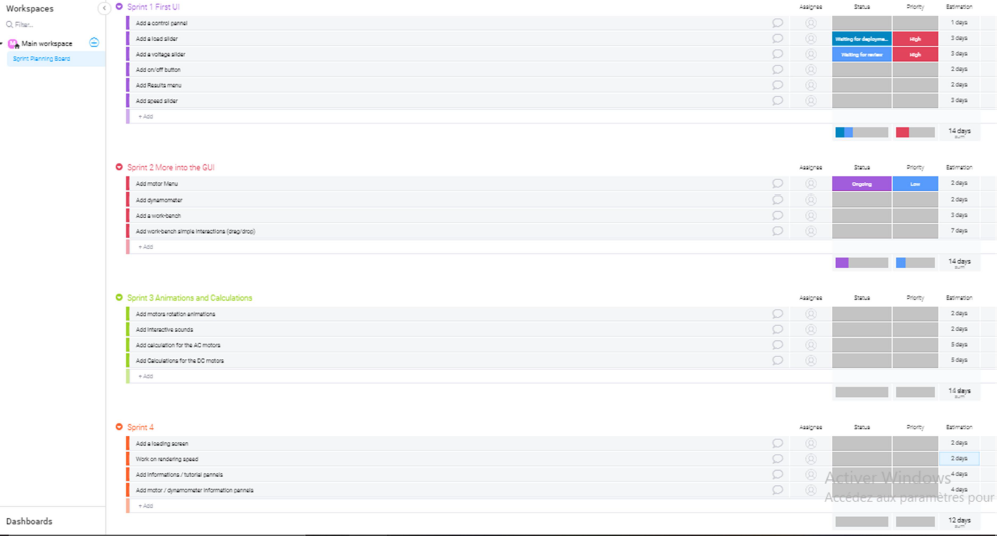
\includegraphics[scale=0.7, frame]{SprintPlanning.png}
		\caption{Sprint planning}
	\end{center}
\end{figure}

\begin{table}[H]
	\begin{center}
	\begin{tabular}{|l|}
		\hline
		\rowcolor[HTML]{6600ff}
		\multicolumn{1}{|c|}{\color{white}\textbf{Sprint name}} \\ \hline
		Sprint 1 : First UI                        \\ \hline
		Sprint 2 : Into the GUI                    \\ \hline
		Sprint 3 : Animations and calculations     \\ \hline
		Sprint 4 : Optimization and final touch    \\ \hline
	\end{tabular}
\end{center}
\caption[Sprints name]{Sprints name}
\end{table}

\section{Task Management}
We used Trello board to manage our tasks.

\begin{figure}[H]
	\begin{center}
		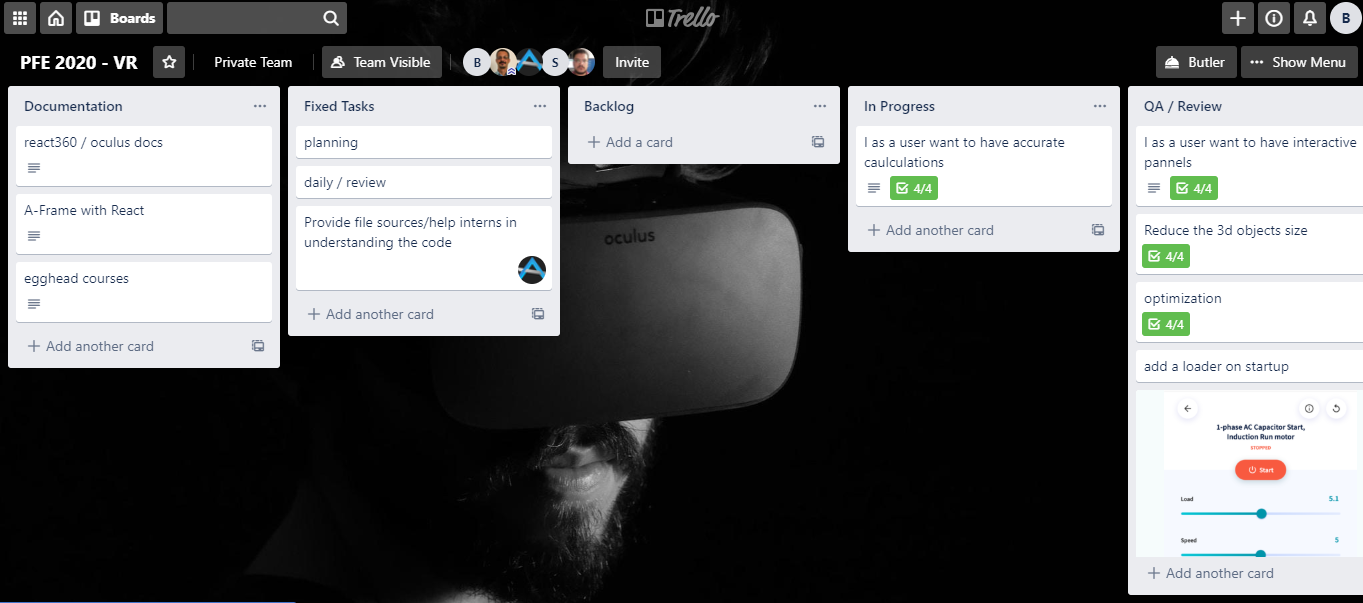
\includegraphics[scale=0.5, frame]{Trello.png}
		\caption{Trello}
	\end{center}
\end{figure}

\section{Functional Requirements Modeling}
\subsection{Use case}

\begin{figure}[H]
		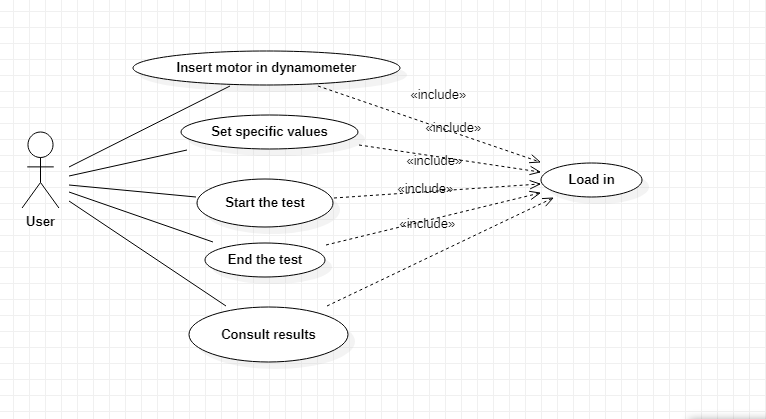
\includegraphics[scale=0.8, frame]{useCase.png}
		\caption{global use case}
\end{figure}

\section{Conclusion}
This chapter explained the work-flow and the approaches
we used to manage the work using an accurate planning and
estimate the time it’s gonna take to deliver the project we
also defined the functional and non-functional aspects of
the application and in the next chapter we will start the
actual work on the project .


\chapter{Project Initialization}
\section{Introduction}
This chapter will desribe the architecture used for the development of the application and than we will discuss the materials used to relaise the project.

\section{Solution Architecture}
//PLACE HOLDER FOR THE SOLUTION ARCHITECTURE


\section{Technologies used}
In this section, we will present the different technologies used to develop our application. The following figure summarizes the development environment used.
\subsection{Hardware environment}
The applications were coded on two Asus laptop computers with the following features:\\
{\indent - Intel(R) core processor ™ i7-7500U CPU @ 2.70 GHZ 2.90 GHZ.}\\
\indent - A RAM of 8 GB.\\
\indent - A 1 Terabyte hard disk drive\\
and tested with oculus quest.
\subsection{Used paltforms}



\begin{wrapfigure}{l}{5.5cm}
	
	\includegraphics[width=5.5cm]{React}
	\caption{React Logo}
\end{wrapfigure}

\textbf{React} is an open-source JavaScript library for building user interfaces. React makes it painless to create interactive UIs using what is known as declarative views it makes the code easier to go through and debug . To summerise , React update and render each component you use while dynamically managing their own state making it fast in terms of performance and able to build complex UIs.\\ \par
\begin{wrapfigure}{l}{5.5cm}
	
	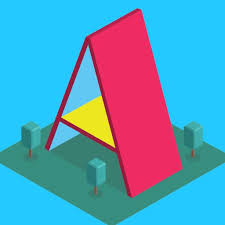
\includegraphics[width=5.5cm]{Aframe}
	\caption{A-frame Logo}
\end{wrapfigure}

\textbf{A-Frame} is a web framework for building virtual reality experiences. Since A-Frame is built on top of the DOM, web libraries such as React, Vue.js, Angular, Ember.js, d3.js are able to sit cleanly on top of A-Frame.

A-Frame is an entity-component-system (ECS) framework exposed through HTML. ECS is a pattern used in game development that favors composability over inheritance, which is more naturally suited to 3D scenes where objects are built of complex appearance, behavior, and functionality. In A-Frame, HTML attributes map to components which are composable modules that are plugged into entity to attach appearance, behavior, and functionality.
\\ \par 

\begin{wrapfigure}{l}{5.5cm}
	
	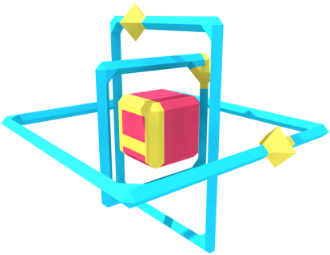
\includegraphics[width=5.5cm]{Aframe-react}
	\caption{Aframe-react Logo}
\end{wrapfigure}
Released on the same day as A-Frame, \textbf{aframe-react} is a very thin layer on top of A-Frame to bridge with React. aframe-react passes React props to directly A-Frame using refs and .setAttribute(), bypassing the DOM. This works since A-Frame's .setAttribute()s are able to take non-string data such as objects, arrays, or elements and synchronously modify underlying 3D scene graph.\\ \par
\begin{wrapfigure}{l}{5.5cm}
	
	
\includegraphics[width=5.5cm]{super-hands}
	\caption{super-hands Logo}
\end{wrapfigure}
\textbf{super-hands} adds natural, intuitive interactions with tracked controller, touch, or mouse input in A-Frame.
The goal of super-hands is to make it easy to handle user input in Web VR by providing a high-level API that is consistent across all devices. Instead of dealing directly with controller button events, raycasters, and collision detection components, you setup your scene and components instead to respond to 'gestures' like hovering and grabbing. \\ \par


\subsection{Tools used}
\subsubsection{Coding tools}


\begin{wrapfigure}{l}{5cm}
	
	
\includegraphics[width=4cm]{vscode}
	\caption{visual studio code Logo}
\end{wrapfigure}
\textbf{Visual Studio Code} is a lightweight but powerful source code editor which runs on your desktop.
Since in our case we manipulate multiple Languages and frameworks it helps conduct all the work in one place and avoid confusion and blockers and its extensions packs allow for multiple customisation options that allow the user to have a smooth work-flow.
 \\ \\\\\par 
 \subsubsection{3D designing tools}
\begin{wrapfigure}{l}{5.5cm}
		
\includegraphics[width=5.5cm]{3dBuilder}
	\caption{3D builder Logo}
\end{wrapfigure} 


\textbf{3D builder} is a Microsoft provided application that allows for viewing , creating and editing 3D objects with a variety of powerfull tools . It also allows to turn simple images into their 3D model with the option to manipulate the content as pleased and it also allows you to build from scratch your desired 3D objects. \\\\\\\\\par

\subsubsection{Versioning tools}
\begin{wrapfigure}{l}{5.5cm}
	
\includegraphics[width=5.5cm]{gitlab}
	\caption{GitLab Logo}
\end{wrapfigure} 

GitLab is a complete open-source DevOps platform, delivered as a single application, fundamentally changing the way Development, Security, and Ops teams collaborate and build software. From idea to production, GitLab helps teams improve cycle time from weeks to minutes, reduce development process costs and decrease time to market while increasing developer productivity.
GitLab helps teams design, develop and securely manage code and project data from a single distributed version control system to enable rapid iteration and delivery of business value. GitLab repositories provide a scalable, single source of truth for collaborating on projects and code which enables teams to be productive without disrupting their workflows.


\subsubsection{Modeling tool}


\begin{wrapfigure}{l}{4cm}
	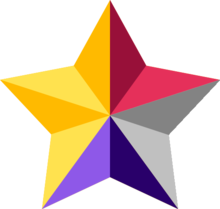
\includegraphics[width=4cm]{Staruml}
	\caption{StarUml Logo}
\end{wrapfigure} 


“StarUML is an open source software-modeling tool that supports UML (Unified Modeling Language). It is based on UML version 1.4, provides eleven different types of diagram and it accepts UML 2.0 notation. It actively supports the MDA (Model Driven Architecture) approach by supporting the UML profile concept and allowing generating code for multiple languages.”  \\\\\\\\\par

\section{Conclusion}

This chapter contained the detailed information on different logical aspects of the development process explaining the tools used and the architecthre decided upon while also expanding reasons toward why we made certain choices as we move forward to the sprints section of this work .

\begin{thebibliography}{9}
	
	\bibitem{lambo}
	Clark Lambot,
	\textit{A Brief History of VR},
	https://veer.tv/blog/a-brief-history-of-vr/,
	8 Nov , 2018.
	
	\bibitem{lambo}
	Clark Lambot,
	\textit{A Brief History of VR},
	https://veer.tv/blog/a-brief-history-of-vr/,
	8 Nov , 2018.
	
	\bibitem{lamport94}
	Leslie Lamport,
	\textit{\LaTeX: a document preparation system},
	Addison Wesley, Massachusetts,
	2nd edition,
	1994.
	
\end{thebibliography}

\end{document}          
